\documentclass[tikz]{standalone}
\usepackage[utf8]{inputenc}
\usepackage{amsmath}
\usetikzlibrary{intersections}

\begin{document}

% parabola and cusp
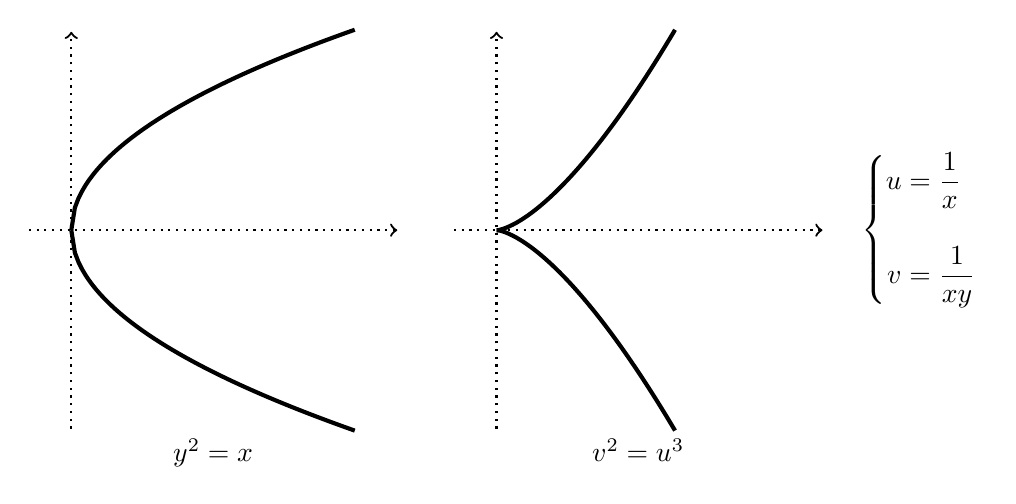
\begin{tikzpicture}[thick,scale=1.8]
\draw[->,dotted] (-.3, 0) -- (2.3,0);
\draw[->,dotted] (0,-1.4) -- (0,1.4);
\path[draw,name path=para1,samples=80,line width=1.5pt,domain=0:2] plot (\x, {sqrt(\x)});
\path[draw,name path=para2,samples=80,line width=1.5pt,domain=0:2] plot (\x, -{sqrt(\x)});
\node[below] at (1,-1.4) {$y^2 = x$};

\begin{scope}[shift={(3,0)}]
\draw[->,dotted] (-.3, 0) -- (2.3,0);
\draw[->,dotted] (0,-1.4) -- (0,1.4);
\path[draw,name path=para1,samples=80,line width=1.5pt,domain=0:1.26] plot (\x, {sqrt(\x^3)});
\path[draw,name path=para2,samples=80,line width=1.5pt,domain=0:1.26] plot (\x, -{sqrt(\x^3)});
\node[below] at (1,-1.4) {$v^2 = u^3$};
\node[right] at (2.5,0) {\hbox{$\left\{\begin{aligned}u &=\frac 1x \\[10pt] v&=\frac{1}{xy}\end{aligned}\right.$}};
\end{scope}

\end{tikzpicture}

\end{document}